\subsection{Decyzje podjęte podczas implementacji}

\subsubsection{Wstęp}

Podczas realizacji projektu zbadano różne podejścia i rozwiązano liczne problemy implementacyjne, aby wdrożyć architekturę opisaną w rozdziale trzecim. Każdy podrozdział omawia po jednym z aspektów – od wymagań do implementacji.

\subsubsection{Komunikacja pomiędzy Elementami Lupus}

Pierwszym krokiem w implementacji było wymyślenie sposobu na komunikację pomiędzy \hyperlink{def:element-lupus}{\textbf{Elementami Lupus}}. Z racji, że \hyperlink{def:element-lupus}{\textbf{Elementy Lupus}} są \textit{Zasobami Własnymi}, wykorzystano tu natywne mechanizmy Kubernetes opisane w podrozdziałach 4.2 i 4.3. Ideą było to, że \textit{Operator} jednego elementu dokonuje zmian w obiekcie API innego elementu, co wywoła ponownie \textit{Operator} elementu ale z innym obiektem wejściowym. \hyperlink{def:element-lupus}{\textbf{Elementy Lupus}} modyfikują nawzajem swój \texttt{Status}, a dokładniej jego pole \texttt{input}, przekazując tam swoją \hyperlink{def:finalne-dane}{\textbf{finalną postać danych}}.

\begin{figure}[!h]
    \centering 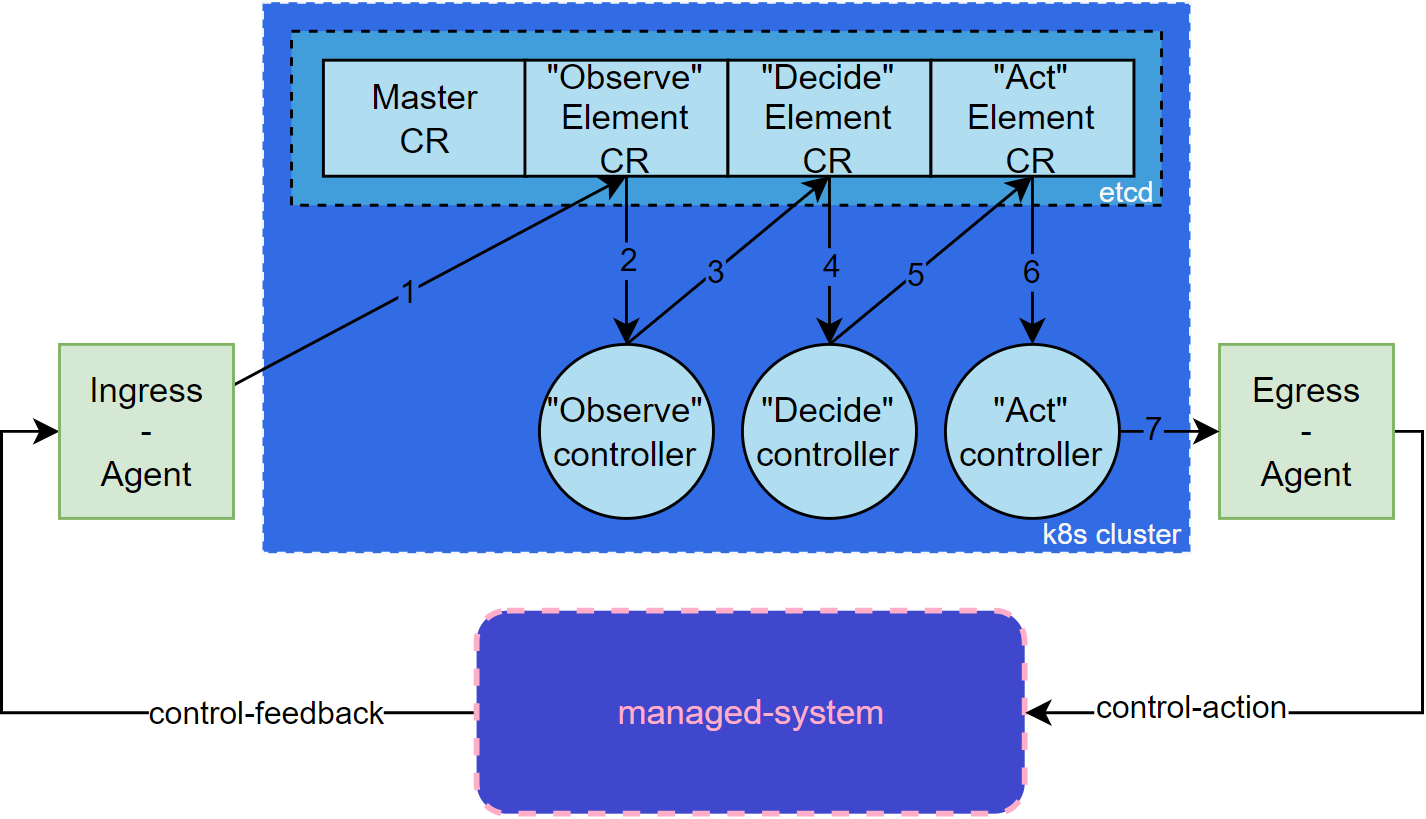
\includegraphics[width=1\linewidth]{43-komunikacja.png}
    \caption{Komunikacja pomiędzy Elementami Lupus. Źródło: Opracowanie własne.}\label{fig:43-komunikacja}
\end{figure}

Sposób działania został ukazany na rysunku \ref{fig:43-komunikacja}. Początkowo \hyperlink{def:element-lupus}{\textbf{Elementy Lupus}} mogły przyjąć postać jednego z trzech typów: Observe, Decide lub Execute\footnote{W myśl okrojonej pętli OODA}. \hyperlink{def:agent-ingress}{\textbf{Agent Ingress}} modyfikował \texttt{Status} obiektu Observe (krok 1). To wywoływało operator elementu "Observe" (krok 2). Operator Observe modyfikował \texttt{Status} obiektu Decide (krok 3). Na koniec modyfikacje otrzymywał obiekt elementu "Act" (krok 5), którego Operator przekazywał swoje \hyperlink{def:dane}{\textbf{Dane}} do \hyperlink{def:agent-egress}{\textbf{Agenta Egress}} (krok 7). 

Z czasem jednak, aby nie narzucać konkretnej struktury pętli, zrezygnowano z trzech typów i stworzono jeden uniwersalny typ, którego Operator jest w stanie wykonać \hyperlink{def:workflow-petli}{\textbf{Workflow Akcji}}, co pozwalało na wyrażenie logiki dowolnego z 3 poprzednich typów. W ten sposób spełniono \hyperref[req:10]{Wymaganie 10}.

\subsubsection{Dane}

\hyperref[req:10]{Wymaganie 10} nakazuje, aby \hyperlink{def:element-lupus}{\textbf{Elementy Lupus}} były sterowane danymi (\textit{data-driven}). \hyperlink{def:dane}{\textbf{Dane}} oraz \hyperlink{def:workflow-petli}{\textbf{Workflow Akcji}} spełniają to wymaganie. Dzięki nim \hyperlink{def:element-lupus}{\textbf{Elementy Lupus}} mogą wykonać dowolny zestaw \hyperlink{def:akcja}{\textbf{Akcji}} na \hyperlink{def:dane}{\textbf{Danych}}, dając \hyperlink{def:projektant}{\textbf{Projektantowi}} pewną elastyczność. To właśnie \hyperlink{def:dane}{\textbf{Dane}} przekazywane są jako pole \texttt{input} w statusie obiektu API \hyperlink{def:element-lupus}{\textbf{Elementu Lupus}}. 

Z racji uniwersalności \hyperlink{def:dane}{\textbf{Danych}}, należało wybrać format, który pozwoli na ich możliwie dużą dowolność. Wybór padł na JSON, ze względu na jego ogólnie przyjęty standard i możliwości reprezentacji dowolnej struktury danych. 

Kubernetes z kolei wymaga, aby pola umieszczane w \texttt{Statusie} Zasobu miały konkretny typ. Dokonano więc analizy, jaki typ nadaje się do reprezentacji obiektu JSON. Wybór padł na \texttt{RawExtension}. Jest to typ zdefiniowany przez zespół Kubernetes, używany do obsługi dowolnych surowych danych w formacie JSON lub YAML. Należy do pakietu \texttt{k8s.io/apimachinery/pkg/runtime} i jest często stosowany, gdy zasób musi osadzić lub pracować ze strukturą danych, która jest elastyczna, ale jednocześnie uporządkowana. \texttt{RawExtension} spełnia te wymagania.

\begin{lstlisting}[language=go, caption={\emph{Definicja struktury Go reprezentującej status Elementu Lupus}}\label{lst:431}]
// ElementStatus defines the observed state of Element
type ElementStatus struct {
	// Input contains operational data
	Input runtime.RawExtension `json:"input"`
	// Timestamp of the last update
	LastUpdated metav1.Time `json:"lastUpdated"`
}
\end{lstlisting}

\texttt{RawExtension} to typ, którego użyjemy do przenoszenia \hyperlink{def:dane}{\textbf{Danych}} między \hyperlink{def:element-lupus}{\textbf{Elementami Lupus}}. Pozostaje kwestia reprezentacji tych \hyperlink{def:dane}{\textbf{Danych}} w Operatorach \hyperlink{def:lupus}{\textbf{Lupus}}. 

\begin{lstlisting}[language=go, caption={\emph{Definicja struktury Go RawExtension w paczce k8s.io/apimachinery/pkg/runtime}}\label{lst:432}]
type RawExtension struct {
    Raw []byte `json:"-"` // Serialized JSON or YAML data
    Object Object         // A runtime.Object representation
}
\end{lstlisting}

Zamierzonym celem \texttt{RawExtension} według deweloperów Kubernetes jest umożliwienie deserializacji do określonej, znanej struktury. Jednak ze względu na \hyperref[req:10]{Wymaganie 10} taka struktura nie istnieje. Potrzebujemy więc natywnej struktury Go, która jest w stanie reprezentować dowolny obiekt JSON. Pierwszym pomysłem, który się nasuwa, jest użycie typu Go \texttt{interface{}}, ponieważ może on reprezentować dowolne dane. Problem z \texttt{interface{}} polega jednak na tym, że nie można na nim operować – nie udostępnia żadnego interfejsu do interakcji. Jest to typ podstawowy.

Drugim pomysłem na reprezentację JSON-a było użycie \texttt{map[string]interface{}}, ponieważ większość instancji JSON-a to faktycznie obiekty klucz-wartość. Klucze w tym przypadku są typu \texttt{string}, a wartości mogą być dowolne (stąd użycie \texttt{interface{}}) w Go. W większości przypadków obiekty JSON zawierają kilka głównych pól (ang. \textit{top-level fields}), co idealnie pasuje do reprezentacji \texttt{map[string]interface{}}.

Tak właśnie narodziło się pojęcie \hyperlink{def:dane}{\textbf{Danych}}. \hyperlink{def:dane}{\textbf{Dane}} to w rzeczywistości struktura opakowująca i dająca odpowiedni interfejs (ang. \textit{Wrapper}) dla wspomnianej wcześniej mapy.

\begin{lstlisting}[language=go, caption={\emph{Definicja struktury Go dla Danych}}\label{lst:433}]
type Data struct {
	Body map[string]interface{}
}
\end{lstlisting}

Ta struktura posiada bogaty zestaw funkcji (metod), które pełnią rolę interfejsu do pracy z \hyperlink{def:dane}{\textbf{Danymi}}. Metody te są wywoływane podczas wykonywania \hyperlink{def:akcja}{\textbf{Akcji}} i zazwyczaj – z wyjątkiem metod \texttt{Get} i \texttt{Set} – każda metoda odpowiada dokładnie jednej akcji. Kluczowym konceptem \hyperlink{def:dane}{\textbf{Danych}} jest \hyperlink{def:pole-danych}{\textbf{Pole Danych}} (ang. \textit{Data-field}). Jest ono odpowiednikiem pola w JSON-ie. Każde pole jest identyfikowane przez swój \hyperlink{def:klucz}{\textbf{Klucz}} i przechowuje wartość. Za pomocą metody \texttt{Get} możemy pobrać wartość znajdującą się pod danym kluczem, a przy użyciu \texttt{Set} możemy ustawić nową wartość dla pola wskazanego określonym kluczem. 

Nie obejmuje to jednak wszystkich obiektów JSON, jakie istnieją. JSON pozwala, aby element na najwyższym poziomie był tablicą. Nakłada to pewne ograniczenia na projektowanie pętli. Szczególnie JSON reprezentujący aktualny stan \hyperlink{def:system-zarzadzany}{\textbf{Systemu Zarządzanego}}, wysyłany przez \hyperlink{def:interfejs-lupin}{\textbf{Interfejs Lupin}}, musi być serializowalny do \texttt{map[string]interface{}}. Oznacza to, że nie może być:
\begin{itemize}
    \item typem prymitywnym,
    \item tablicą,
    \item obiektem JSON z kluczami innymi niż \texttt{string}.
\end{itemize}

Warto zaznaczyć, że nazwa „Dane” nawiązuje do definicji przedstawionej we wstępie historycznym. Dopiero komponenty zewnętrzne względem platformy Lupus, czyli elementy systemu zarządzania wyposażone w mechanizmy sztucznej inteligencji, będą przekształcać dane pochodzące z systemu zarządzanego w informacje lub wiedzę.

Dla platformy, która pełni jedynie funkcję orkiestratora workflow pętli sterowania, dane pozostają transparentne. Nazwa „Dane” podkreśla ich surową formę, wskazując, że platforma nie dokonuje ich interpretacji ani przetwarzania.

\subsubsection{Polimorfizm w Go}

Notacja \textbf{LupN} pozwala, aby wiele jej obiektów posiadało swój typ. Przykładowo akcje są różnorakiego typu. Mają pewną część wspólną, ale też pola szczególne dla każdego typu. Go jest statycznie typowanym językiem, który nie posiada dziedziczenia ani tradycyjnego obiektowego polimorfizmu. Dlatego dokonano analizy jak w Go osiągnąć tę wielopostaciowość.

\textbf{Polimorfizm poprzez interfejsy}

Natywnym sposobem na polimorfizm w Go jest ten osiągany poprzez interfejsy. To zagadnienie najlepiej tłumaczy poniższy kod.


\begin{lstlisting}[language=go, caption={\emph{Przykład polimorfizmu poprzez interfejsy}}\label{lst:434}]
package main

import (
	"fmt"
)

type Forwarder interface {
	Forward() string
}

type NextElement struct {
	Name string
}

func (e *NextElement) Forward() string {
	return fmt.Sprintf("Forwarding to element: %s", e.Name)
}

type Destination struct {
	URL string
}

func (d *Destination) Forward() string {
	return fmt.Sprintf("Forwarding to destination: %s", d.URL)
}

func ProcessForwarder(f Forwarder) {
	fmt.Println(f.Forward())
}

func main() {
	element := &NextElement{Name: "Element1"}
	destination := &Destination{URL: "https://example.com"}

	ProcessForwarder(element)
	ProcessForwarder(destination)
}
\end{lstlisting}

\textbf{Schemat działania}

\begin{itemize}
    \item \textbf{Definicja interfejsu:}  
    \texttt{Forwarder} definiuje metodę \texttt{Forward()}, którą muszą zaimplementować określone typy.
    
    \item \textbf{Konkretne implementacje:}  
    \texttt{NextElement} oraz \texttt{Destination} implementują metodę \texttt{Forward()}.
    
    \item \textbf{Zastosowanie:}  
    Każdy typ spełniający interfejs \texttt{Forwarder} może być przekazywany do funkcji oczekujących obiektu \texttt{Forwarder}.
\end{itemize}

\textbf{Polimorfizm poprzez wskaźniki oraz pole dyskryminatora}

Kolejnym potężnym i idiomatycznym wzorcem w Go jest \textbf{polimorfizm w stylu Go z użyciem wskaźników}, gdzie struktura posiada opcjonalne pola wskaźnikowe, a pole \texttt{type} (dyskryminator) określa, które z tych pól jest istotne w czasie działania programu.

\begin{lstlisting}[language=go, caption={\emph{Przykład polimorfizmu poprzez wskaźniki oraz pole dyskryminatora}}\label{lst:435}]
type Next struct {
	// Type specifies the type of next loop-element
	Type string `json:"type"`
	// List of input keys (Data fields) that have to be forwarded
	Keys []string `json:"keys"`
	// One of the fields below is not null
	Element     *NextElement `json:"element,omitempty"`
	Destination *Destination `json:"destination,omitempty"`
}

type NextElement struct {
	Name string `json:"name"`
}

type Destination struct {
	URL string `json:"url"`
}

func (n *Next) Validate() error {
	if n.Type == "element" && n.Element == nil {
		return fmt.Errorf("Element must be set 
        for type 'element'")
	}
	if n.Type == "destination" && n.Destination == nil {
		return fmt.Errorf("Destination must be set 
        for type 'destination'")
	}
	if n.Element != nil && n.Destination != nil {
		return fmt.Errorf("Only one of Element 
        or Destination can be set")
	}
	return nil
}
\end{lstlisting}

\textbf{Schemat działania}

\textbf{Unia tagowana} to wzorzec, w którym pole \texttt{tag} określa, którą z kilku możliwych reprezentacji danych wykorzystuje dany obiekt. W Go jest to realizowane poprzez kombinację:

\begin{itemize}
    \item Pole dyskryminujące typ (np. \texttt{Type string}).
    \item Pola wskaźnikowe dla możliwych wariantów. Jeśli dane pole nie występuje w aktualnej reprezentacji obiektu, jego wartość jest po prostu \texttt{nil}.
    \item Podczas działania programu możemy zweryfikować, której reprezentacji danych używa obiekt, i odpowiednio na tej podstawie podjąć działanie.
\end{itemize}

Podczas działania programu możemy zweryfikować, której reprezentacji danych używa obiekt, i odpowiednio na tej podstawie podjąć działanie.

\textbf{Porównanie}

Porównanie zostało przedstawione w tabeli \ref{tab:431}

\begin{table}[h!]
\centering
\renewcommand{\arraystretch}{1.5} % Zwiększenie odstępów między wierszami
\begin{tabular}{|p{4cm}|p{5.5cm}|p{5.5cm}|}
\hline
\textbf{Funkcja}               & \textbf{Polimorfizm przez wskaźniki}                                   & \textbf{Polimorfizm przez interfejsy}                          \\ \hline
\textbf{Zachowanie w czasie działania} & Używa dyskryminatora (\texttt{Type}) i pól wskaźnikowych           & Używa implementacji metod do polimorfizmu                     \\ \hline
\textbf{Bezpieczeństwo typów}      & Wymaga jawnej walidacji                                              & Wymuszane podczas kompilacji za pomocą interfejsów            \\ \hline
\textbf{Serializacja}          & Bezproblemowa z JSON                                                 & Może wymagać niestandardowego \texttt{marshaling}             \\ \hline
\textbf{Rozszerzalność}        & Dodaj nowe pola wskaźnikowe i zaktualizuj enum \texttt{Type}          & Dodaj nowe typy implementujące interfejs                      \\ \hline
\textbf{Łatwość użycia}         & Prosta, ale wymaga ręcznej walidacji                                 & Czysta i idiomatyczna w Go                                    \\ \hline
\textbf{Wspólne zachowanie}    & Wymaga zewnętrznej logiki                                            & Enkapsulowane w metodach interfejsu                           \\ \hline
\end{tabular}
\caption{Porównanie polimorfizmu przez wskaźniki i przez interfejsy w Go.}\label{tab:431}
\end{table}

Polimorfizm przez wskaźniki oferuje przejrzystą reprezentację danych, która jest łatwo serializowana i deserializowana do formatu JSON lub YAML. Dodatkowo wspiera włączenie pola \texttt{type} jako części modelu danych, dzięki czemu może być ono również przechowywane lub przesyłane. Z drugiej strony polimorfizm przez interfejsy jest natywny dla Go, bardziej czytelny i zapewnia silne sprawdzanie typów podczas kompilacji.

\textbf{Podsumowanie:}

\begin{itemize}
    \item Polimorfizm przez wskaźniki jest preferowany w aplikacjach skoncentrowanych na danych.
    \item Polimorfizm przez interfejsy jest preferowany w aplikacjach skoncentrowanych na zachowaniach.
\end{itemize}

W \hyperlink{def:lupus}{\textbf{Lupus}} polimorfizm był potrzebny do reprezentacji różnych typów (odmian) niektórych \hyperlink{def:element}{\textbf{Obiektów LupN}}, takich jak \hyperlink{def:akcja}{\textbf{Actions}} lub \hyperlink{def:next}{\textbf{Next}}, dlatego wybrano polimorfizm poprzez wskaźniki oraz pole dyskryminatora.

\subsubsection{Dwa rodzaje workflow}\label{sec:dwa-rodzaje-workflow}

W \hyperlink{def:lupus}{\textbf{Lupus}} występują dwa rodzaje \textit{workflow}: \hyperlink{def:workflow-petli}{\textbf{Workflow Pętli}}, które definiuje przepływ pracy \hyperlink{def:element-lupus}{\textbf{Elementów Lupus}}, oraz \hyperlink{def:workflow-petli}{\textbf{Workflow Akcji}}, które definiuje przepływ \hyperlink{def:akcja}{\textbf{Akcji}} we wnętrzu pojedynczego elementu. Występują między nimi pewne różnice w możliwościach, wynikające ze sposobu implementacji komunikacji między ich węzłami.

\begin{itemize}
    \item Węzły w \hyperlink{def:workflow-petli}{\textbf{Workflow Pętli}} komunikują się ze sobą poprzez pobudzanie operatorów.
    \item Węzły w \hyperlink{def:workflow-petli}{\textbf{Workflow Akcji}} komunikują się poprzez pamięć RAM zaalokowaną przez pojedynczy operator \hyperlink{def:element-lupus}{\textbf{Elementu Lupus}}.
\end{itemize}

Różnice są widoczne w specyfikacji LupN w \hyperlink{appendix:3}{Załączniku 3}.

\subsubsection{Funkcje użytkownika}\label{sec:funkcje-uzytkownika}

Zgodnie z \hyperref[req:7]{Wymaganiem 7}, \hyperlink{def:element-lupus}{\textbf{Elementy Lupus}} nie wykonują \hyperlink{def:czesc-obliczeniowa}{\textbf{Części Obliczeniowej Logiki Pętli}}. Zamiast tego, jest ona delegowana do \hyperlink{def:element-zewnetrzny}{\textbf{Elementów Zewnętrznych}}.

W tym kontekście pojawiają się dwa kluczowe zagadnienia:
\begin{itemize}
    \item Jak ma postępować \hyperlink{def:uzytkownik}{\textbf{Użytkownik}} w sytuacji, gdy konieczne jest wykonanie prostej operacji na \hyperlink{def:dane}{Danych} (np. dodanie dwóch wartości), a wdrażanie dedykowanego serwera HTTP okazuje się nieopłacalne?
    \item Każda platforma ramowa (ang. \textit{framework}) powinnna być rozszerzalna.
\end{itemize}

Z tych dwóch powodów wdrożono mechanizm o nazwie „Definiowane przez użytkownika, wewnętrzne funkcje Go”, określany w skrócie jako \hyperlink{def:funkcje-uzytkownika}{\textbf{Funkcje Użytkownika}}.

\hyperlink{def:uzytkownik}{\textbf{Użytkownik}} może definiować własne fragmenty kodu Go jako funkcje i wywoływać je jako jedną z \hyperlink{def:destynacja}{\textbf{Destynacji}} w akcji \hyperlink{def:akcja}{\textbf{Send}}.

W repozytorium kodu z projektem Kubebuilder znajduję plik o nazwie \texttt{user-functions.go} \footnote{\url{https://github.com/0x41gawor/lupus/blob/master/lupus/internal/controller/user-functions.go}}. To w nim \textbf{Użytkownik} może definiować swoje funkcje. Plik posiada jedną przykładową funkcję.

\begin{lstlisting}[language=go, caption={\emph{Przykładowa funkcja użytkownika}}\label{lst:436}]
// Exemplary user-function. It just returns the input
func (UserFunctions) Echo(input interface{}) (interface{}, error) {
	return input, nil
}
\end{lstlisting}

Funkcja jako argument przyjmuje \texttt{interface{}}, który będzie reprezentował \textbf{pole danych}.\footnote{Pola lub pól, gdyż pod tym pojęciem może też się kryć użycie "*"}. Zwracanym typem jest również \texttt{interface{}}, ponieważ wartość zwracana przez element zewnętrzny zostaje wpisana do \textbf{pola danych}.

Nazwa \texttt{UserFunctions} jest strukturą, która gromadzi funkcje użytkownika.

\begin{lstlisting}[language=go, caption={\emph{Stukrutra składują funckje użytkowniak jako swoje metody.}}\label{lst:437}]
// UserFunctions struct for user-defined, internal functions
type UserFunctions struct{}
\end{lstlisting}

Pojawia się zatem pytanie, jak wywołać taką funkcję w notacji \hyperlink{def:lupn}{\textbf{LupN}}. Na szczęście funkcje w Go mogą być używane jako typy i przechowywane jako  co umożliwia ich zapis w strukturze mapy klucz-wartość, gdzie nazwy funkcji (typ \texttt{string}) pełnią rolę kluczy.


\begin{lstlisting}[language=go, caption={\emph{Mapa przechowująca funkcje użytkownika}}\label{lst:438}]
// A global map to store function references
var FunctionRegistry = map[string]func(input interface{}) (interface{}, error){}
\end{lstlisting}

Następnie, z pomocą biblioteki \texttt{reflect}\footnote{\url{https://pkg.go.dev/reflect}} można zaimplementować funkcję, która iteruje po metodach struktury \texttt{UserFunctions} i zapisuje je do powyższej mapy jako wartości, dla których kluczami są nazwy funkcji. 

\begin{lstlisting}[language=go, basicstyle=\ttfamily\tiny, caption={\emph{Funkcja zapełniająca mapę funkcji użytkownika}}\label{lst:439}]
// RegisterFunctions dynamically registers user-defined functions
func RegisterFunctions(target interface{}) {
	t := reflect.TypeOf(target)
	v := reflect.ValueOf(target)

	for i := 0; i < t.NumMethod(); i++ {
		method := t.Method(i)

		// Ensure the method matches the required signature
		if method.Type.NumIn() == 2 && // Receiver + input
			method.Type.NumOut() == 2 && // Output + error
			method.Type.In(1).Kind() == reflect.Interface && // Input: interface{}
			method.Type.Out(0).Kind() == reflect.Interface && // Output: interface{}
			method.Type.Out(1).Implements(reflect.TypeOf((*error)(nil)).Elem()) { // Second output: error

			funcName := method.Name
			FunctionRegistry[funcName] = func(input interface{}) (interface{}, error) {
				// Call the user-defined function
				result := method.Func.Call([]reflect.Value{v, reflect.ValueOf(input)})

				// Handle result[1] (error) being nil
				var err error
				if !result[1].IsNil() {
					err = result[1].Interface().(error)
				}

				return result[0].Interface(), err
			}
		}
	}
}
\end{lstlisting}

Funkcja widoczna na listingu \ref{lst:439} jest wywoływana podczas inicjalizacji paczki kontrolera z strukturą \texttt{UserFunctions} jako argument.

\begin{lstlisting}[language=go, caption={\emph{Inicjaliza mapy}}\label{lst:4310}]
func init() {
	// Fill in the FunctionRegistry map 
	// with functions defined as a method of UserFunctions{}
	RegisterFunctions(UserFunctions{})
}
\end{lstlisting}


Od tego momentu, dana funkcja może zostać wywołana po nazwie w funkcji obsługującej akcję Send w interpreterze Operatora Elementu Lupus.

\begin{lstlisting}[language=go, caption={\emph{Wywołąnie funkcji użytkownika w akcji send}}\label{lst:4311}]
func sendToGoFunc(funcName string, body interface{}) (interface{}, error) {
	if fn, exists := FunctionRegistry[funcName]; exists {
		return fn(body)
	} else {
		return nil, fmt.Errorf("no such UserFunction defined")
	}
}
\end{lstlisting}

W notacji \textbf{LupN} wystarczy zapis:

\begin{lstlisting}[language=sh, caption={\emph{Użycie funkcji użytkownika w LupN}}\label{lst:4312}]
  - name: "bounce"
    type: send
    send:
        inputKey: "field1"
        destination:
        type: gofunc
        gofunc:
            name: echo
        outputKey: "field2"
\end{lstlisting}